\section*{Methods}
% In the Methods section, you should describe the implementation and architectural details of your system - in particular, this addresses how you approached the problem and the design of your solution. For those who believe in reproducible science, this should be fine-grained enough such that somebody could implement your model/algorithm and reproduce the results you claim to achieve.

\begin{figure}[H]
	\centering
	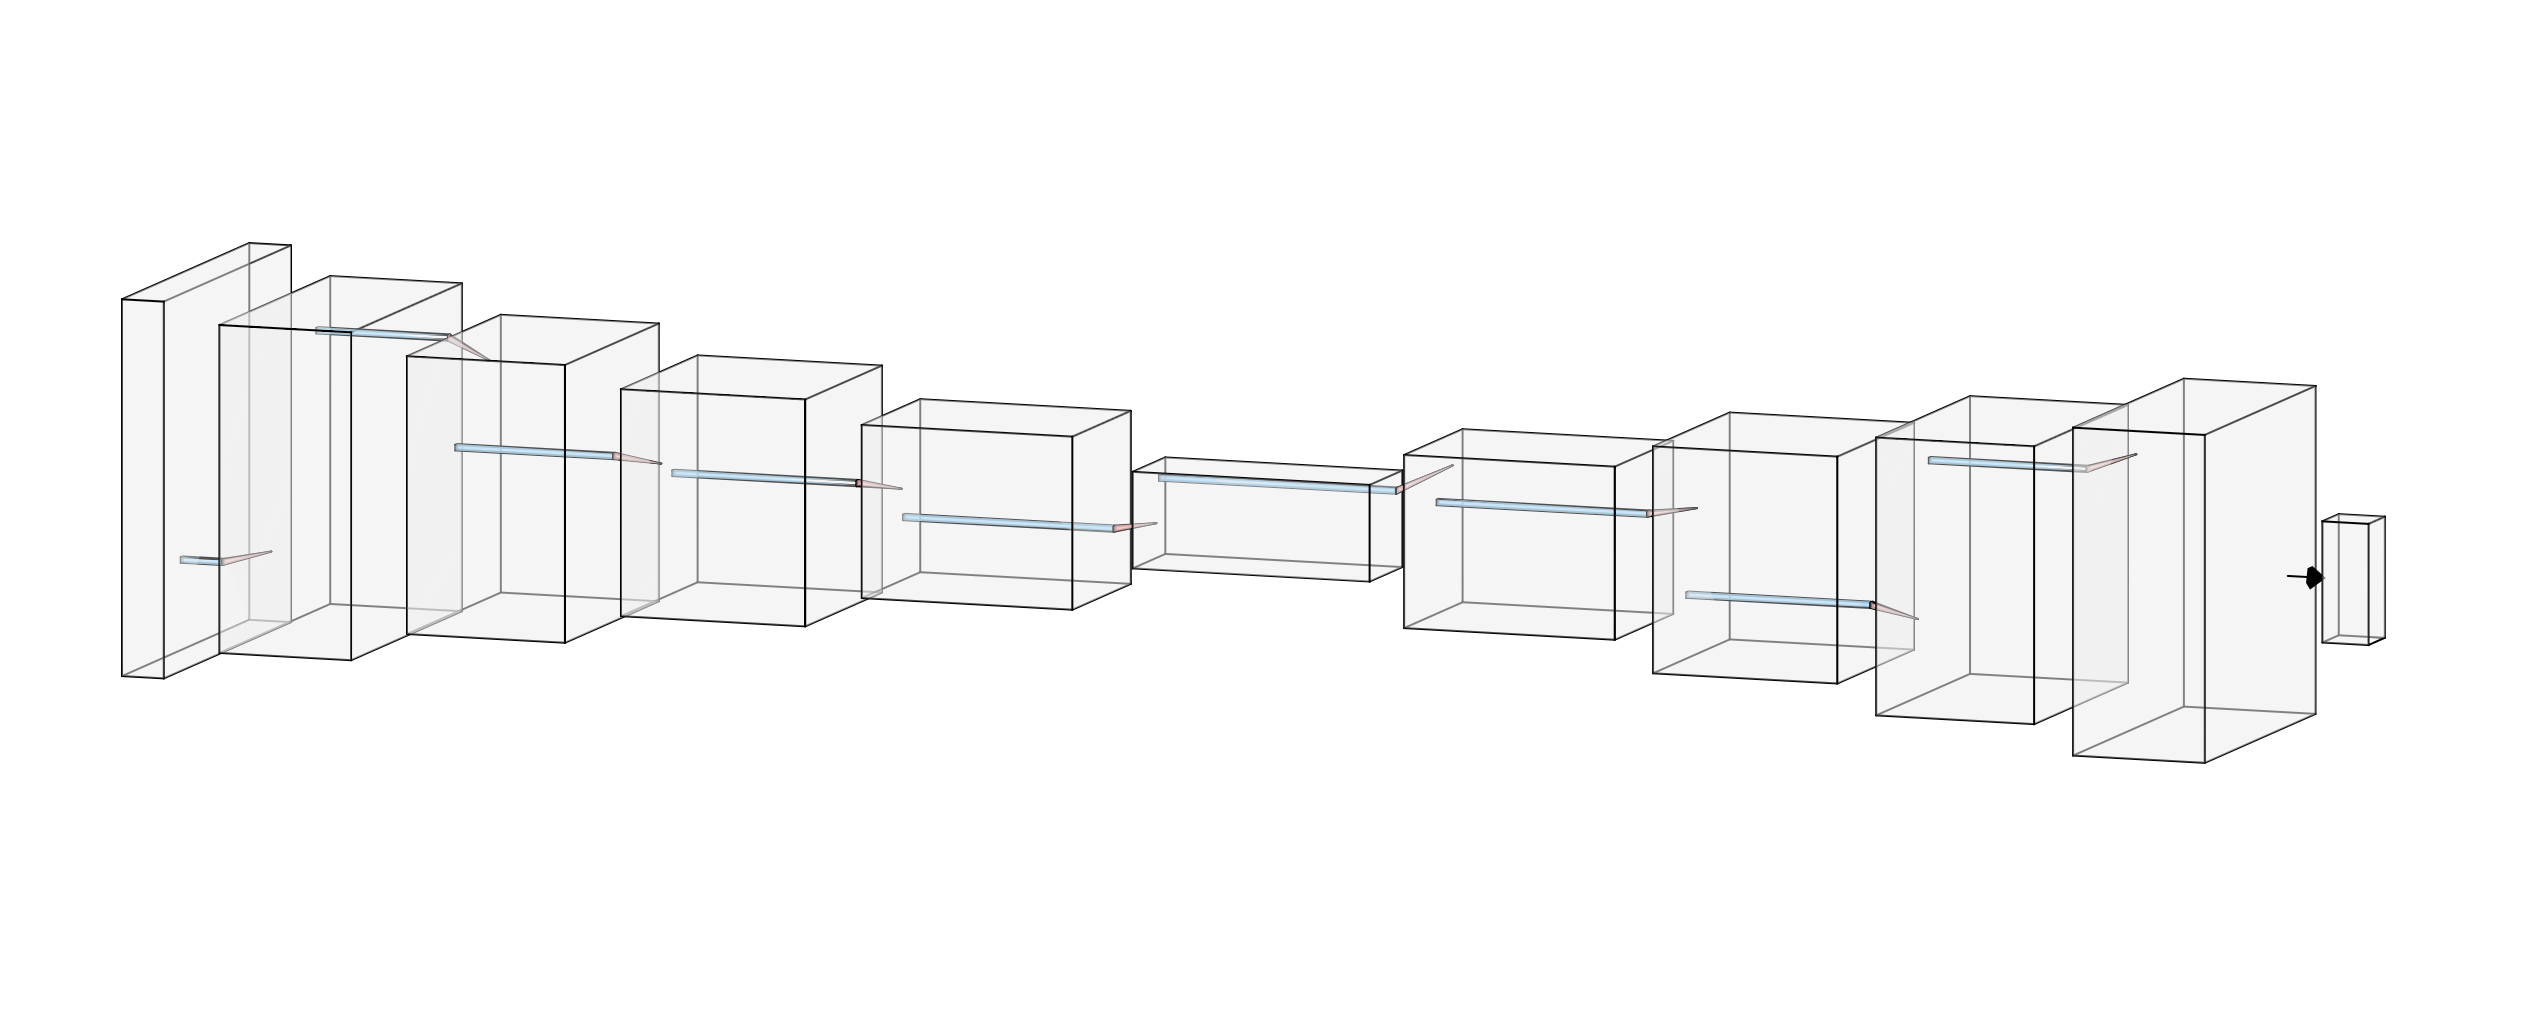
\includegraphics[width=\textwidth]{images/architecture}
	\caption{Visualization of System Architecture}
	\label{fig:architecture}
\end{figure}

\section*{Baseline}
% (a) Baseline (5 pt): You should describe the baseline architecture, stating the appropriate activation function on the last layer of the network, the loss criterion, weights initialization scheme and the gradient descent optimizer you used.
Our baseline architecture consists of an encoder, decoder, classifier, and activation. We used the Adam gradient descent optimizer

\subsubsection*{Encoder}
We have five convolutional layers that increases the depth of the orginal 3 channels to 32 to 64 to 128 to 256 to 512 each using a size 3 kernel, padding of 1, a stride of 2, and no dilation. Each layer sees a small decrease in the height and width of the layer according to the expression $\frac{W - F + 2P}{2} + 1$. The outputs of each convolutional layer are subsequently passed through a ReLU activation function and a batch normalization layer.

\subsubsection*{Decoder}
We have five deconvolutional, or upsampling layers that decreases the depth of the final 512 deep layer output from the encoder. This is decreases from 512 to 256 to 128 to 64 to 32 each using a size 3 kernel, padding of 1, a stride of 2, and no dilation. Each layer sees a small decrease in the height and width of the layer according to the expression $S(W - 1) + F - 2P$. Similarly, the outputs of each deconvolutional layer are subsequently passed through a ReLU activation function and a batch normalization layer.

\subsubsection*{Classifier and Activation}
In our final layer, we have a $1 \times 1$ convolutional kernel working as a classifier, and a softmax activation layer. This layer projects a probability distribution stream over the 21 classes.

\section*{Improvements Over Baseline}
% (b) Improvements over Baseline (5 pt): You should describe the approaches you took to improve over the baseline model.

\subsubsection*{Data Augmentation}
To enhance the robustness of our model, we applied data augmentation techniques to our dataset. This involved performing various transformations on the input images, such as mirror flips, rotations, and crops. During the process, we must ensure that the same transformations are applied to the corresponding labels to maintain data integrity throughout the augmentation process. We found that data augmentation improved on the average Jaccard index on our models by around 0.03-0.05.

\subsubsection*{Cosine Annealing}
In order to optimize the learning rate dynamically throughout the training process, we implemented the cosine annealing learning rate scheduler. This technique adjusts the learning rate in a cosine-shaped manner, effectively annealing it towards zero as training progresses. By aligning the learning rate adjustments with the number of epochs, we aim to improve the convergence and generalization capabilities of our model. Training our models with cosine annealing had a minimal improvement in both our accuracy and Jaccord index.

\subsubsection*{Class Imbalance}
To mitigate the challenges posed by class imbalance, particularly addressing rare classes, we employed strategies to alleviate this issue. One approach is to apply a weighted loss criterion, which assigns higher weights to the infrequent classes during the optimization process. By doing so, we incentivize the network to pay more attention to these underrepresented classes, thus improving its ability to accurately classify them. Otherwise, the model could simply learn to label the entire image the background and still achieve decent pixel accuracy. The introduction of weight decay had a considerable improvement in our Jaccard index and was used in all our models moving on.

\section*{Experimentation}

% (c) Experimentation (10 pt): Describe your two experimental CNN architectures(parts 5.a and 5.b) and the U-Net, each in a table, which the first column indicate the particular layer of your network, and the other columns state the layer’s dimensions (e.g. in-channels, out-channels, kernel-size, padding/stride) and activation function/non-linearity. Describe any regularization techniques (e.g. data augmentation) you used, parameter initialization methods, gradient descent optimization, and how you addressed the class-imbalance problem .
In this work, we introduce DarrenNet, a novel architecture inspired by the erfnet architecture but distinguished by its enhanced efficiency and superior performance. Leveraging a modified erfnet structure, DarrenNet incorporates additional convolution layers and employs higher dropout, resulting in a more intricate and efficient network. The augmented convolutional layers contribute to a deeper understanding of spatial features, while increased dropout aids in regularization, preventing overfitting. The fusion of these modifications yields a model that not only operates more efficiently but also achieves superior performance in various tasks. We are also able to use pretrained erfnet encoders, which improve our performance further.

Below are the descriptions (in table format) and regularization techniques used for each architecture.

\subsection*{DarrenNet Architecture}
\begin{table}[H]
	\centering
	\label{tab:darrenyu}
	\setlength{\abovecaptionskip}{10pt}
	\begin{tabular}{|c|c|c|c|c|c|c|}
		\hline
		\textbf{Layer}    & \textbf{In} & \textbf{Out} & \textbf{Padding} & \textbf{Kernel} & \textbf{Stride} & \textbf{Activation} \\ \hline
		Initial Block     &             & 16           & 0                & 3x3             & 1               & ReLU                \\ \hline
		Downsampler 1     & 16          & 64           & 0                & 3x3             & 2               & ReLU                \\ \hline
		Non-bottleneck 1  & 64          & 64           & 0                & 3x3             & 1               & ReLU                \\ \hline
		Non-bottleneck 2  & 64          & 64           & 0                & 3x3             & 1               & ReLU                \\ \hline
		Non-bottleneck 3  & 64          & 64           & 0                & 3x3             & 1               & ReLU                \\ \hline
		Non-bottleneck 4  & 64          & 64           & 0                & 3x3             & 1               & ReLU                \\ \hline
		Non-bottleneck 5  & 64          & 64           & 0                & 3x3             & 1               & ReLU                \\ \hline
		Downsampler 2     & 64          & 128          & 0                & 3x3             & 2               & ReLU                \\ \hline
		Non-bottleneck 6  & 128         & 128          & 0                & 3x3             & 1               & ReLU                \\ \hline
		Non-bottleneck 7  & 128         & 128          & 0                & 3x3             & 1               & ReLU                \\ \hline
		Non-bottleneck 8  & 128         & 128          & 0                & 3x3             & 1               & ReLU                \\ \hline
		Non-bottleneck 9  & 128         & 128          & 0                & 3x3             & 1               & ReLU                \\ \hline
		Non-bottleneck 10 & 128         & 128          & 0                & 3x3             & 1               & ReLU                \\ \hline
		Non-bottleneck 11 & 128         & 128          & 0                & 3x3             & 1               & ReLU                \\ \hline
		Non-bottleneck 12 & 128         & 128          & 0                & 3x3             & 1               & ReLU                \\ \hline
		Non-bottleneck 13 & 128         & 128          & 0                & 3x3             & 1               & ReLU                \\ \hline
		Upsampler 1       & 128         & 64           & 0                & 3x3             & 1               & ReLU                \\ \hline
		Non-bottleneck 14 & 64          & 64           & 0                & 3x3             & 1               & ReLU                \\ \hline
		Non-bottleneck 15 & 64          & 64           & 0                & 3x3             & 1               & ReLU                \\ \hline
		Upsampler 2       & 64          & 16           & 0                & 3x3             & 1               & ReLU                \\ \hline
		Non-bottleneck 16 & 16          & 16           & 0                & 3x3             & 1               & ReLU                \\ \hline
		Non-bottleneck 17 & 16          & 16           & 0                & 3x3             & 1               & ReLU                \\ \hline
		Output Conv       & 16          & 21           & 0                & 2x2             & 2               & -                   \\ \hline
	\end{tabular}
	\caption{DarrenNet Architecture}
\end{table}

\begin{table}[H]
	\setlength{\abovecaptionskip}{10pt}
	\centering
	\begin{tabular}{|l|c|c|c|c|c|c|}
		\hline
		\textbf{Layer Name} & \textbf{In}          & \textbf{Out}         & \textbf{Padding}      & \textbf{Kernel Size} & \textbf{Stride} & \textbf{Activation} \\
		\hline
		conv1               & $n_{\text{channel}}$ & $n_{\text{channel}}$ & (1, 0)                & 3x1                  & 1               & ReLU                \\
		\hline
		conv2               & $n_{\text{channel}}$ & $n_{\text{channel}}$ & (0, 1)                & 1x3                  & 1               & ReLU                \\
		\hline
		conv3               & $n_{\text{channel}}$ & $n_{\text{channel}}$ & (1$\times$dilated, 0) & 3x1                  & 1               & ReLU                \\
		\hline
		conv4               & $n_{\text{channel}}$ & $n_{\text{channel}}$ & (0, 1$\times$dilated) & 1x3                  & 1               & ReLU                \\
		\hline
		bn1                 &                      &                      &                       &                      &                 &                     \\
		\hline
		bn2                 &                      &                      &                       &                      &                 &                     \\
		\hline
		dropout             &                      &                      &                       &                      &                 & 2D                  \\
		\hline
	\end{tabular}
	\caption{Non-bottleneck (DarrenNet)}
\end{table}

\begin{table}[H]
	\setlength{\abovecaptionskip}{10pt}
	\centering
	\begin{tabular}{|l|c|c|c|c|c|c|}
		\hline
		\textbf{Layer Name} & \textbf{In}            & \textbf{Out}                                 & \textbf{Padding} & \textbf{Kernel Size} & \textbf{Stride} & \textbf{Activation} \\
		\hline
		conv                & $in_{\text{channel}}$  & $out_{\text{channel}} - in_{\text{channel}}$ & 1                & 3x3                  & 2               &                     \\
		\hline
		pool                &                        &                                              &                  & 2x2                  & 2               &                     \\
		\hline
		bn                  & $out_{\text{channel}}$ & $out_{\text{channel}}$                       &                  &                      &                 &                     \\
		\hline
	\end{tabular}
	\caption{DownsamplerBlock (DarrenNet)}
\end{table}

\begin{table}[H]
	\setlength{\abovecaptionskip}{10pt}
	\centering
	\begin{tabular}{|l|c|c|c|c|c|c|}
		\hline
		\textbf{Layer Name} & \textbf{In}            & \textbf{Out}           & \textbf{Padding} & \textbf{Kernel Size} & \textbf{Stride} & \textbf{Activation} \\
		\hline
		conv                & $in_{\text{channel}}$  & $out_{\text{channel}}$ & (1, 1)           & 3x3                  & 2               &                     \\
		\hline
		bn                  & $out_{\text{channel}}$ & $out_{\text{channel}}$ &                  &                      &                 &                     \\
		\hline
	\end{tabular}
	\caption{UpsamplerBlock (DarrenNet)}
\end{table}

\subsection*{DarrenNet Techniques}
In our DarrenNet architecture, we use horizontal and vertical flipping, Kaiming weight initialization, cosine annealing, and add extra penalty to loss inversely proportional to the frequency of a given class pixel.

\subsection*{Transfer Learning Architecture}
\begin{table}[H]
	\centering
	\label{tab:transfer}
	\setlength{\abovecaptionskip}{10pt}
	\begin{tabular}{|c|c|c|c|c|c|c|}
		\hline
		\textbf{Layer} & \textbf{In} & \textbf{Out} & \textbf{Padding} & \textbf{Kernel} & \textbf{Stride} & \textbf{Activation} \\ \hline
		encoder        &             &              &                  &                 &                 &                     \\ \hline
		deconv1        & 512         & 256          & 1                & 3x3             & 2               & ReLU                \\ \hline
		deconv1        & 512         & 256          & 1                & 3x3             & 2               & ReLU                \\ \hline
		deconv2        & 256         & 128          & 1                & 3x3             & 2               & ReLU                \\ \hline
		deconv3        & 128         & 64           & 1                & 3x3             & 2               & ReLU                \\ \hline
		deconv4        & 64          & 32           & 1                & 3x3             & 2               & ReLU                \\ \hline
		conv           & 32          & 21           & 1                & 3x3             & 2               & Softmax             \\ \hline
	\end{tabular}
	\caption{Transfered Encoder to Basic FCN Architecture}
\end{table}

\subsection*{Transfer Learning Techniques}
% In transfer learning, we use horizontal and vertical flipping, Kaiming weight initialization, cosine annealing, and add extra penalty to loss inversely proportional to the frequency of a given class pixel.

\subsection*{UNet Architecture}
\begin{table}[H]
	\centering
	\label{tab:unet}
	\setlength{\abovecaptionskip}{10pt}
	\begin{tabular}{|c|c|c|c|c|c|c|}
		\hline
		\textbf{Layer} & \textbf{In} & \textbf{Out} & \textbf{Padding} & \textbf{Kernel} & \textbf{Stride} & \textbf{Activation} \\ \hline
		conv1          & 3           & 64           & 1                & 3x3             & 1               & ReLU                \\ \hline
		conv2          & 64          & 64           & 1                & 3x3             & 1               & ReLU                \\ \hline
		pool1          & 64          & 64           & 0                & 2x2             & 2               &                     \\ \hline
		conv3          & 64          & 128          & 1                & 3x3             & 1               & ReLU                \\ \hline
		conv4          & 128         & 128          & 1                & 3x3             & 1               & ReLU                \\ \hline
		pool2          & 128         & 128          & 0                & 2x2             & 2               &                     \\ \hline
		conv5          & 128         & 256          & 1                & 3x3             & 1               & ReLU                \\ \hline
		conv6          & 256         & 256          & 1                & 3x3             & 1               & ReLU                \\ \hline
		pool3          & 256         & 256          & 0                & 2x2             & 2               &                     \\ \hline
		conv7          & 256         & 512          & 1                & 3x3             & 1               & ReLU                \\ \hline
		conv8          & 512         & 512          & 1                & 3x3             & 1               & ReLU                \\ \hline
		pool4          & 512         & 512          & 0                & 2x2             & 2               &                     \\ \hline
		conv9          & 512         & 1024         & 1                & 3x3             & 1               & ReLU                \\ \hline
		conv10         & 1024        & 1024         & 1                & 3x3             & 1               & ReLU                \\ \hline
		deconv1        & 1024        & 512          & 0                & 2x2             & 2               & ReLU                \\ \hline
		conv11         & 1024        & 512          & 1                & 3x3             & 1               & ReLU                \\ \hline
		conv12         & 512         & 512          & 1                & 3x3             & 1               & ReLU                \\ \hline
		deconv2        & 512         & 256          & 0                & 2x2             & 2               & ReLU                \\ \hline
		conv13         & 512         & 256          & 1                & 3x3             & 1               & ReLU                \\ \hline
		conv14         & 256         & 256          & 1                & 3x3             & 1               & ReLU                \\ \hline
		deconv3        & 256         & 128          & 0                & 2x2             & 2               & ReLU                \\ \hline
		conv15         & 256         & 128          & 1                & 3x3             & 1               & ReLU                \\ \hline
		conv16         & 128         & 128          & 1                & 3x3             & 1               & ReLU                \\ \hline
		deconv4        & 128         & 64           & 0                & 2x2             & 2               & ReLU                \\ \hline
		conv17         & 64          & 64           & 1                & 3x3             & 1               & ReLU                \\ \hline
		conv18         & 64          & 64           & 1                & 3x3             & 1               & ReLU                \\ \hline
		output         & 64          & 21           & 0                & 1x1             & 1               & ReLU                \\ \hline
	\end{tabular}
	\caption{UNet Architecture}
\end{table}

\subsection*{UNet Techniques}
% In the unet architecture, we use horizontal and vertical flipping, Kaiming weight initialization, cosine annealing, and add extra penalty to loss inversely proportional to the frequency of a given class pixel.
